\documentclass[10pt,conference,compsocconf]{IEEEtran}

\usepackage[round]{natbib}
\usepackage[utf8]{inputenc}
\usepackage{hyperref}
\usepackage{graphicx}
\usepackage{subcaption}
\usepackage{amsmath}
\usepackage{bm}
\usepackage{tikz}
\usepackage{tikz-qtree}
\usepackage{amsmath}
\usepackage{amssymb}
\usepackage{amsfonts}
\usepackage{amsthm}
\usepackage{mathrsfs}
\usepackage{cleveref}
\usepackage{xcolor}
\usepackage{gensymb}
\usepackage{float}
\usepackage{textcomp}
\newcommand{\todo}[1]{\textcolor{red}{TODO: #1}}
\pagestyle{plain}
\begin{document}
\title{Machine Learning --- Project 2 --- Road Segmentation}

\author{
  Jean-Baptiste Cordonnier (224633), Arno Schneuwly (223498), Joey Zenhäusern (226652)\\
  \textit{School of Computer and Communication Sciences, EPFL, Switzerland}
}

\maketitle

\begin{abstract}
  In this report, we introduce our implementation of a convolutional U-Net to classify roads on Earth satellite images. Convolutions and transposed convolutional layers are used to capture local image information, we added dilated convolutions to augment the receptive field of our network. An extensive data augmentation process improved the rotation invariance property of our convolutional networks and showed significant enhancement on evaluation images. We achieved a 93.9 F1 score on half of the Kaggle's evaluation dataset. The training took 8 hours on one recent GPU.
\end{abstract}

\section{Introduction}

Given a set of satellite images from Google Maps, as well as ground-truth images where each pixel is labelled as either road or background, we designed a classifier to differentiate roads from other objects on these images. Our training set contains 100 images of size $400\times400$ and associated ground truth where roads are white and background pixels are black. The evaluation dataset contains 100 images of size $608\times608$ and our predictions are evaluated at a $16\times16$ patch level, not at the pixel level. We use a voting and threshold mechanism to make a decision at patch level.

In section~\ref{sec:baseline} and~\ref{sec:unet}, we will present the models we developed to solve this problem. Sections~\ref{sec:augmentation}, \ref{sec:ensemble} and \ref{sec:implementation} focus on data augmentation and tricks that we used to improve precision and recall. Finally, section~\ref{sec:results} and \ref{sec:discussion} give an outline of our results and discuss about other work on image segmentation.

\section{Baseline Model}\label{sec:baseline}

We used the baseline provided with the project statement. It runs classification on $16\times16$ patches with 2 convolution layers, ReLU activation function and 2 fully connected layers to predict binary class probability. Using this approach yields a 0.804 F1 score on half of the evaluation. The main limitation of this baseline is the lack of context of neighboring pixels. It has trouble recognizing bigger objects than cars and is fooled by any local obstruction, such as trees or bridges. Furthermore, the base line quantize the ground truth into $16\times16$ patches and thus lose some local information regarding the sharp boarders of the roads. On the other hand, it has the advantage to be trained on the exact same objective function than the evaluation objective (patch classification).

\section{U-Net}\label{sec:unet}

We implemented a U-Net neural network inspired by the work of~\cite{unet} on biomedical image segmentation. The architecture is depicted in \cref{fig:unet}. Our implementation is generalized for color images, arbitrary input size and parameterizable number of layers/filters. We explored different architectures: 4, 5 or 6 layers and filters of size $3\times3$ or $5\times5$. We use $3\times3$ convolution filters and ReLU activation which results in the case of a 5 layer U-net architecture in a total of $2\cdot 10^8$ trainable \texttt{float32} parameters. With valid border parameter, each convolution layer of our U-Net reduces the size of the image by approximately half of the filter width. A network with $l$ layers significantly reduces the size of an input image of width $p_i$ to $p_o=p_i-12\cdot2^{l-1}+8$.

\begin{figure}
  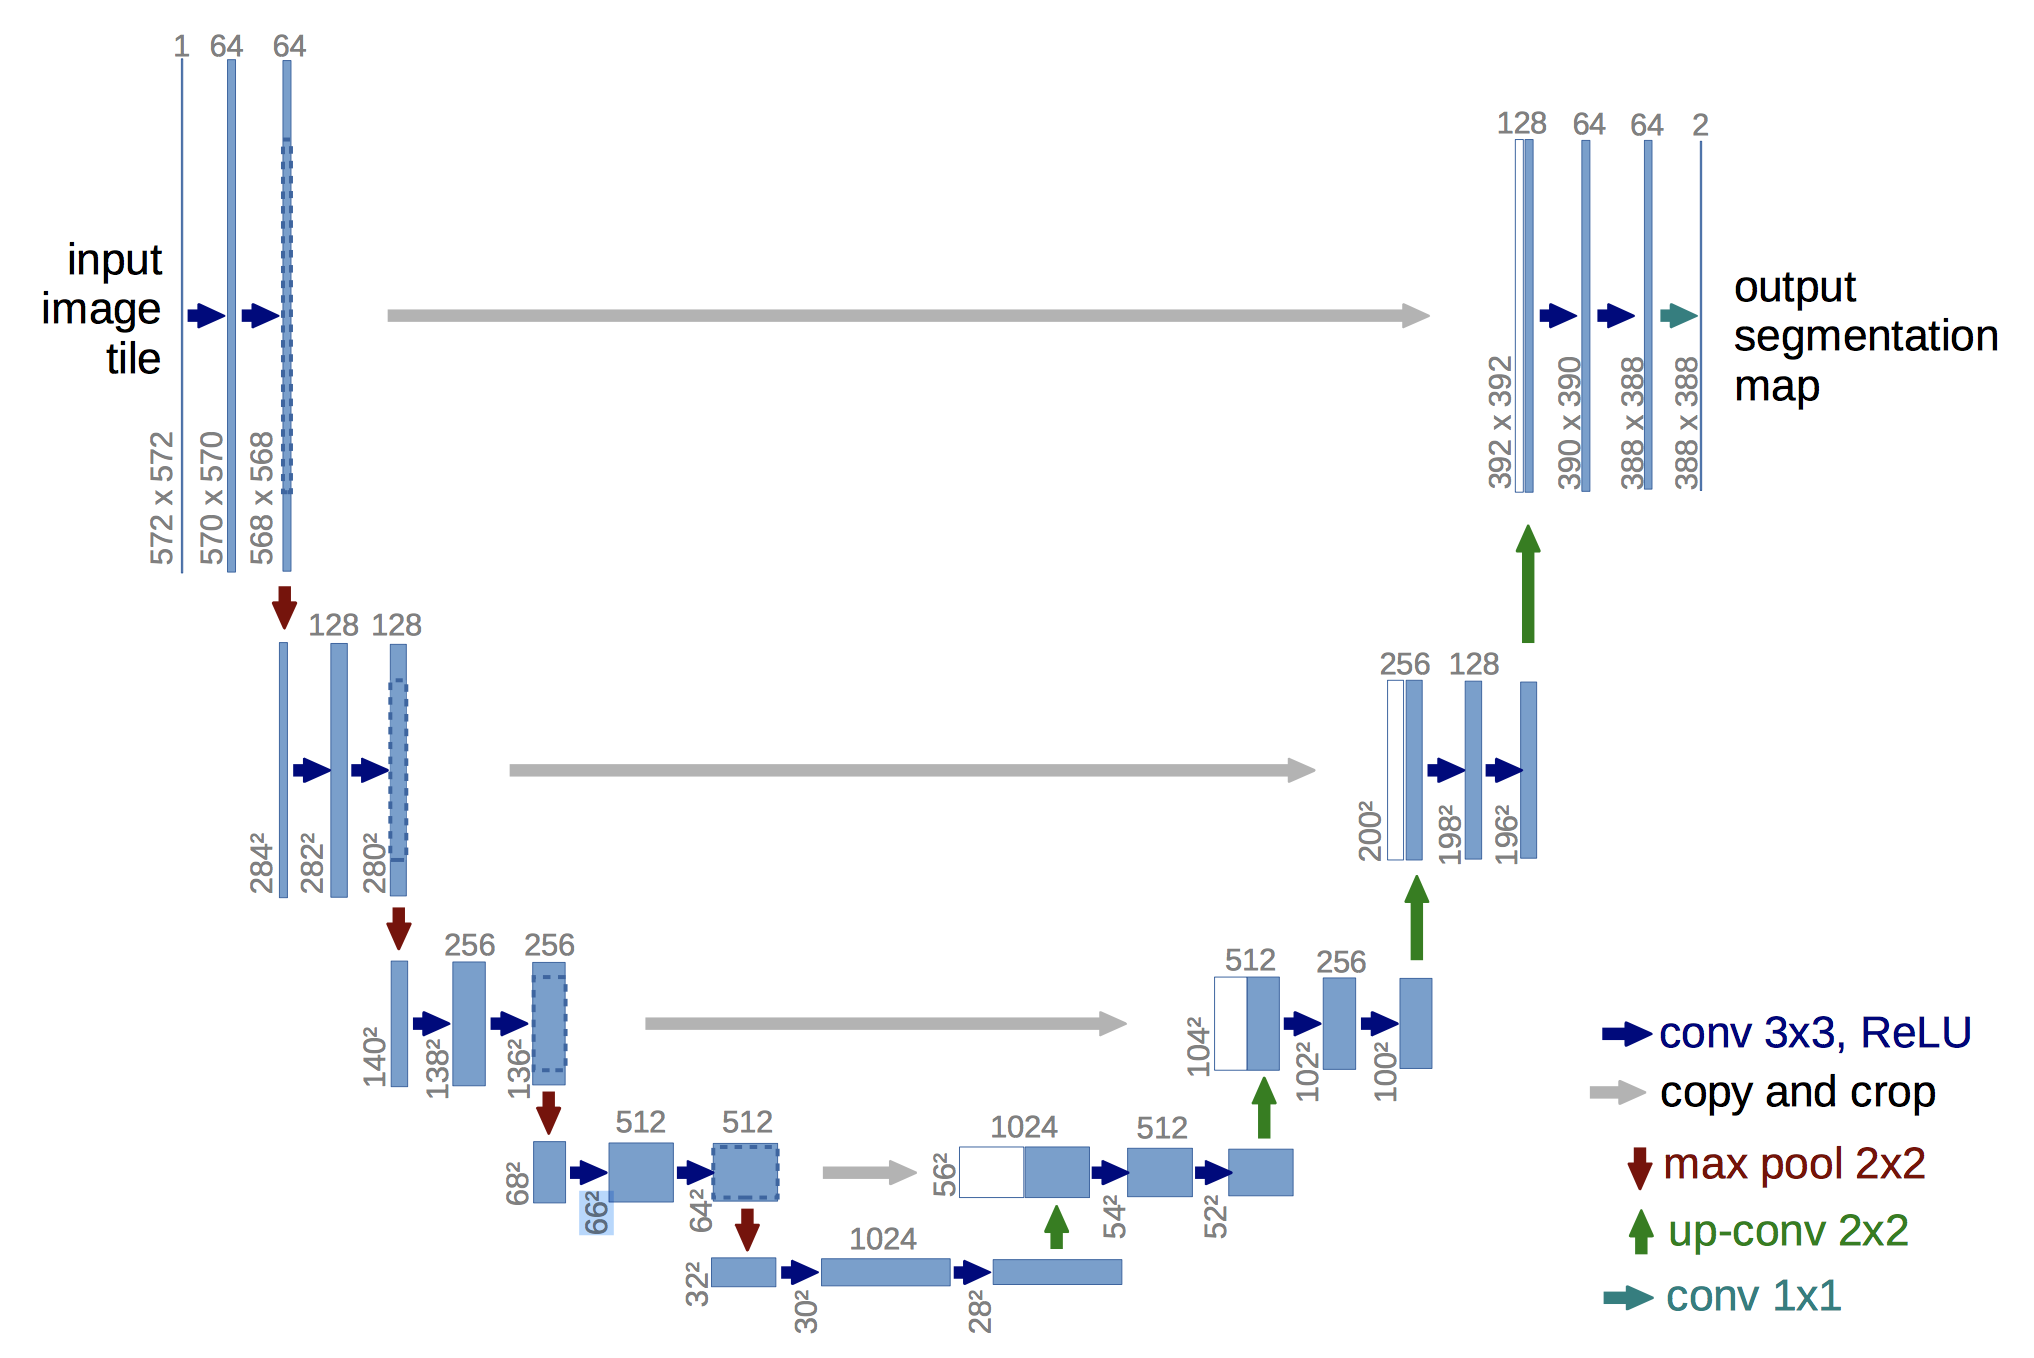
\includegraphics[width=0.95\columnwidth]{figures/unet.png}
  \caption{U-Net architecture from~\cite{unet}\label{fig:unet}}
\end{figure}

The output of the network is a tensor of shape $1\times388\times388\times2$, in other words we have 2 logits per pixel associated to each class (road or background). Note that we stick with a batch size of 1 in order to lower the memory consumption and predict on larger images with more trainable parameters. The binary cross entropy loss is optimized after softmax. We tried to use Adam optimizer (\citealp{kingma2014adam}) but it did not improve convergence time over a basic momentum SGD with exponential decaying learning rate (decay rate 0.95 and step down every 1000 iterations).

To predict a given patch we threshold each pixel's estimated probability of being a road at 0.5 and threshold the proportion of $16\times16$ road pixels by 0.25. This two stages thresholding is motivated by the fact that BCE loss should punish road and background errors symmetrically and secondly the patch ground-truth was derived from pixel ground-truth with cutoff ratio 0.25 (according to the baseline implementation).

Furthermore, we added dropout layers on the input of each convolutional block. We observed a speed up in training time with an keep probability parameter of $0.8$ set arbitrarily.

Analyzing the predicted images, we noticed that challenging situations included roads covered by trees, very thin roads, non-roads that are visually similar to roads (e.g.\ train tracks) as can be seen in \cref{fig:train_eval}. Moreover, the errors mostly happened on tricky parts of the image where a lot of context is needed to infer the pixel's class. For instance, pixels of a road below a railway bridge cannot be classified using only the nearby pixels, it needs to see the global pattern of the image and identify the long road lines (that should be continuous stretches).

That is the reason why we added dilated convolution filters (see \cref{fig:dilated}) at each crop shortcut layer. Dilated convolutions are similar to normal convolutions, but the filter is applied to points that are not contiguous on the image. Each one is separated from its neighbors by a fixed distance called rate, and they form a grid of evenly spaced points. With 2 layers and a dilation rate of 2, we get some information from neurons 4 pixels away instead of 2. In future work, we want to add a pyramidal hierarchy and combine different rates (e.g. PSPNet of \citealp{PSPNet}) to let the model pick the right focus, but for the obtained result we used dilatation rate 2.

\begin{figure}
  \center%
  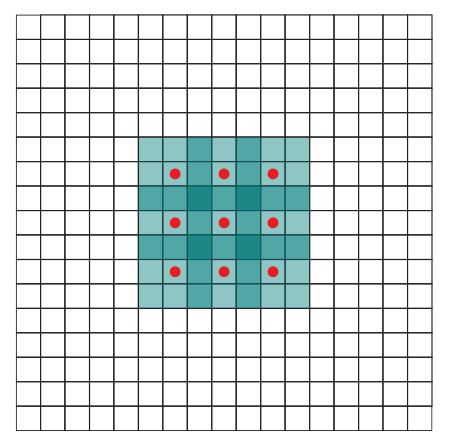
\includegraphics[width=0.5\columnwidth]{figures/dilated.png}
  \caption{Dilated convolution filter from~\cite{ferenc-dilated}}\label{fig:dilated}
\end{figure}


\section{Data Augmentation}\label{sec:augmentation}
Convolutional Neural Networks are known to be translation-invariant but sensitive to rotation. Given that our training dataset for this task is rather small (100 images), we were worried to overfit to these samples. The U-Net model is very powerful and could simply learn all the training images, but we want it to learn patterns and generalize well to unseen images. That is why we decided to artificially augment our dataset during the training, in order to better capture the roads' geometry.
The most intuitive example which justifies such a procedure is the low number of pictures with diagonal streets in the training set. By providing rotated versions of all the training pictures by different angles,  diagonal streets should eventually be captured well.

\subsection{Rotation}\label{sec:rotation}
Our framework provides a function for rotating the images. We feed the training process with the original images and the images rotated by angles of $\{15, 30, 45, 60, 75\}$ degrees. This results in a training set size of 600 images. The other angles within this 15 degree step logic are inferred by the transformations applied by the stochastic image augmentation during the training itself.

\subsection{Mirroring \& Image Patches}
Based on \citep{unet} the image input size of our network is $572\times572$ pixels. The dataset provides training images with size $400\times400$ and the test set images with size $608\times608$. In the case of the training images, a rotation of 45 degrees increases the image width and height by a factor of $\sqrt{2}$, resulting in a version with remaining unfilled corners, even when cropping back to a size of $400\times400$. We do not want to leave these corners empty and have to extend the image in an appropriate way.

The image output size of the network is $388\times388$ pixels, which means that a prediction is only produced for the center of the image. The $572\times572$ patches are generated such that all pixels of the original images appear at least once in the center of the network input image. Centered pixels are not cut off by the convolutions and all pixels of the training and test images are taken into consideration at least once over all the patches. The resulting probabilities of overlapping pixels are averaged.

Therefore, the patching requires the input size of the training and test images to be extended. Combined with the extension requirement through the unfilled corners caused in the rotated versions, we augment the image size accordingly. The augmentation symmetrically mirrors the required amount of pixels at every border. We believe this approach is better than considering the unfilled corners as background or filling them with white noise.

Given an original image of width $w$, an input patch size $p_i$ and a prediction patch size $p_o$, the number of pixel to expand on each side of the original image is shown on \cref{fig:patch} and computed in \cref{eq:expansion}.

\begin{equation}
  \text{expansion} = \underbrace{\frac 1 2 w(\sqrt 2 - 1)}_{45^\circ \text{ rotation gap}} + \underbrace{\sqrt 2 \cdot \frac{p_o - p_i} 2}_{\text{CNN margin removal}}
  \label{eq:expansion}
\end{equation}

\begin{figure}
    \centering
    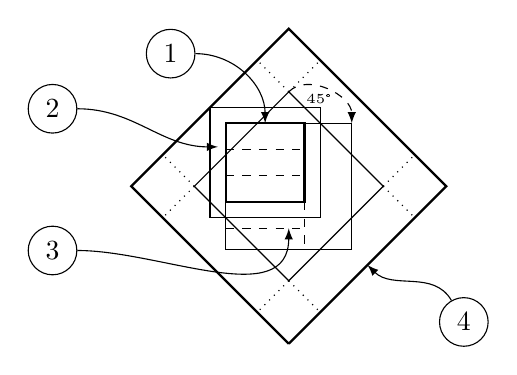
\begin{tikzpicture}
        % big rectangle
        \draw[thick] (2, 0) -- (0, 2) -- (2, 4) -- (4, 2) -- (2, 0);
        % label
        \node[circle, draw=black, anchor=north west] (mirror) at (4, 0.5) {4};
        % arrow
        \draw[-latex] (mirror) to[out=120, in=-45] (3, 1);

        % red rectangle
        \draw (2, 0.8) -- (0.8, 2) -- (2, 3.2) -- (3.2, 2) -- (2, 0.8);

        % dotted lines inside big square
        \draw[dotted] (2, 0.8) -- (1.6, 0.4);
        \draw[dotted] (2, 0.8) -- (2.4, 0.4);

        \draw[dotted] (0.8, 2) -- (0.4, 1.6);
        \draw[dotted] (0.8, 2) -- (0.4, 2.4);

        \draw[dotted] (2, 3.2) -- (1.6, 3.6);
        \draw[dotted] (2, 3.2) -- (2.4, 3.6);

        \draw[dotted] (3.2, 2) -- (3.6, 1.6);
        \draw[dotted] (3.2, 2) -- (3.6, 2.4);

        % inner thick rectangle
        \draw[thick] (1.2, 1.8) -- (1.2, 2.8) -- (2.2, 2.8) -- (2.2, 1.8) -- (1.2, 1.8);
        % label
        \node[circle, draw=black, anchor=north] (patch) at (0.5, 4) {1};
        % arrow
        \draw[-latex] (patch) to[out=0, in=90] (1.7, 2.8);

        % inner thin rectangle
        \draw (1, 1.6) -- (1, 3) -- (2.4, 3) -- (2.4, 1.6) -- (1, 1.6);
        % label
        \node[circle, draw=black, anchor=north, align=left] (cutoff) at (-1, 3.3) {2};
        % arrow
        \draw[-latex] (cutoff) to[out=0, in=180] (1.1, 2.5);

        % extension inner thick rectangle
        \draw (2.2, 2.8) -- (2.8, 2.8) -- (2.8, 1.2) -- (1.2, 1.2) -- (1.2, 1.8);

        % dashed stride outer
        \draw[dashed] (2.2, 1.8) -- (2.2, 1.2);
        \draw[dashed] (1.2, 1.4666) -- (2.2, 1.4666);

        % label
        \node[circle, draw=black, anchor=north, align=left] (next) at (-1, 1.5) {3};
        % arrow
        \draw[-latex] (next) to[out=0, in=-90] (2, 1.4666);

        % arrow 45°
        \draw[-latex, dashed] (2, 3.2) to[out=45, in=90] (2.8, 2.8) node[anchor=south east, inner sep=7pt] {\tiny{45\textdegree}};

        % dashed stride inner
        \draw[dashed] (1.2, 2.1333) -- (2.2, 2.1333);
        \draw[dashed] (1.2, 2.4666) -- (2.2, 2.4666);
        % \node[circle, draw=black, align=left] (stride) at (4, 3.3) {5};
        % \draw[-latex] (stride) to[out=-90, in=-90] (2, 2.6);

    \end{tikzpicture}
    \caption{(1) Inner patch to predict (2) Patch expansion for CNN margin cutoff (3) Next patch after slide of stride pixels (dotted) (4) Original image expanded with mirroring}
    \label{fig:patch}
\end{figure}

\subsection{Stochastic Image Augmentation}\label{sec:aug}
In order to cover all possible rotations and flips over the axes in a memory efficient manner, we only apply 15 degree rotations within the first 90 degrees, as mentioned in section~\ref{sec:rotation}. For easier transformations which only require a matrix flip or transpose, we apply them online with random probability (uniform distribution):

\begin{itemize}
  \item flip upside down or left right with half probability,
  \item diagonal transposition with probability half,
  \item rotation by an angle in $\{0,90,180,270\}$ degrees.
\end{itemize}

This stochastic image augmentation happens directly in the Tensorflow graph and can be deactivated with a
flag placeholder during evaluation.

\subsection{Other transformations}
As the provided training and test images are all of the same quality and high resolution, we decided not to apply other transformations, such as blurring, adding noise, changing contrast or luminosity. Random dilatations are often used in medical image segmentation and are known to help the training a lot. We think that it is not a good fit for road segmentation where the learning would be hurt by seeing malformed roads that cannot exist in reality.

\begin{figure}
    \centering
    \begin{subfigure}[b]{0.3\columnwidth}
      \caption*{Image 23}
        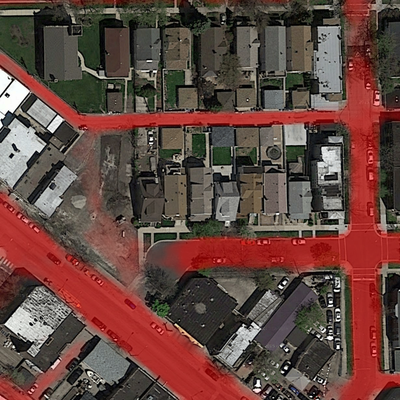
\includegraphics[width=\columnwidth]{figures/training_hard/eval_overlays_pred_002.png}
    \end{subfigure}
    \begin{subfigure}[b]{0.3\columnwidth}
    \caption*{Image 42}
        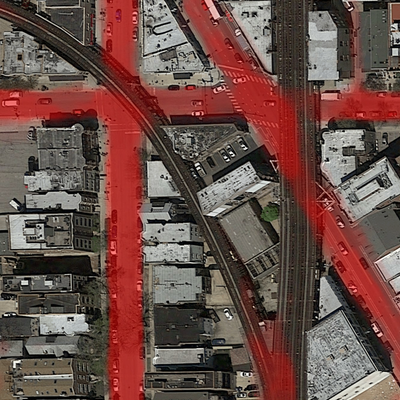
\includegraphics[width=\textwidth]{figures/training_hard/eval_overlays_pred_003.png}
    \end{subfigure}
    \begin{subfigure}[b]{0.3\columnwidth}
    \caption*{Image 91}
        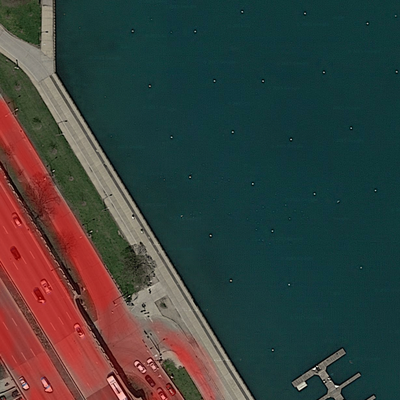
\includegraphics[width=\textwidth]{figures/training_hard/eval_overlays_pred_004.png}
    \end{subfigure}

     \vspace{0.1cm}
    \begin{subfigure}[b]{0.3\columnwidth}
      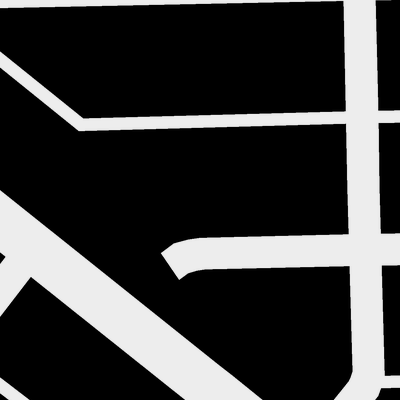
\includegraphics[width=\columnwidth]{figures/training_hard/gt_002.png}
    \end{subfigure}
    \begin{subfigure}[b]{0.3\columnwidth}
      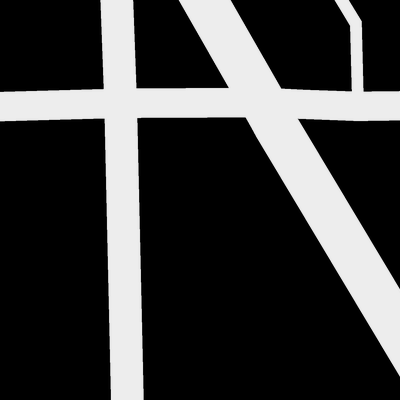
\includegraphics[width=\columnwidth]{figures/training_hard/gt_003.png}
    \end{subfigure}
    \begin{subfigure}[b]{0.3\columnwidth}
      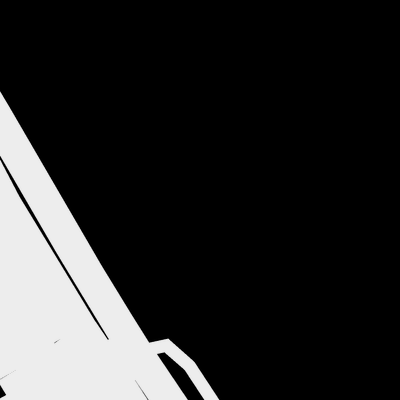
\includegraphics[width=\columnwidth]{figures/training_hard/gt_004.png}
    \end{subfigure}

    \vspace{0.1cm}
    \begin{subfigure}[b]{0.3\columnwidth}
      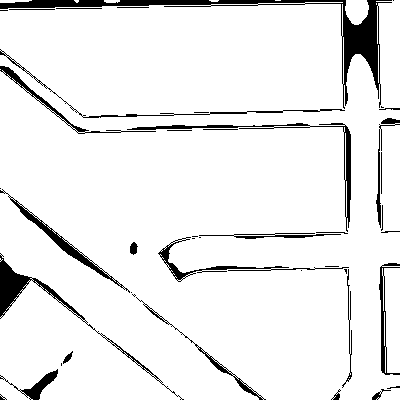
\includegraphics[width=\columnwidth]{figures/training_hard/eval_orror_002.png}
    \end{subfigure}
    \begin{subfigure}[b]{0.3\columnwidth}
      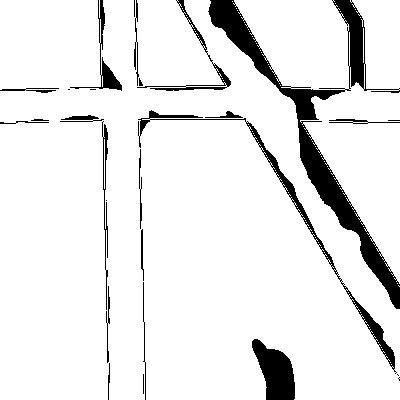
\includegraphics[width=\columnwidth]{figures/training_hard/eval_orror_003.png}
    \end{subfigure}
    \begin{subfigure}[b]{0.3\columnwidth}
      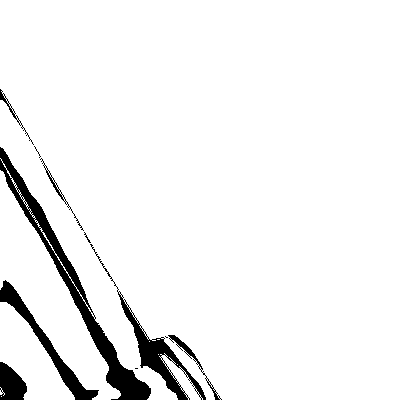
\includegraphics[width=\columnwidth]{figures/training_hard/eval_orror_004.png}
    \end{subfigure}

    \vspace{0.1cm}
    \begin{subfigure}[b]{0.3\columnwidth}
      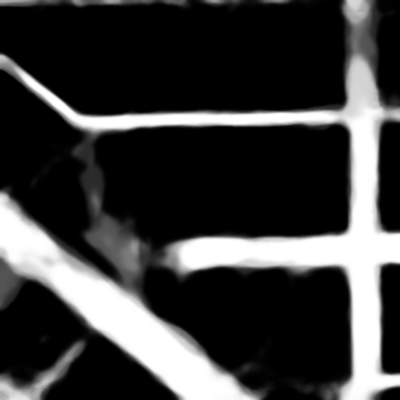
\includegraphics[width=\columnwidth]{figures/training_hard/eval_probability_pred_002.png}
    \end{subfigure}
     \begin{subfigure}[b]{0.3\columnwidth}
      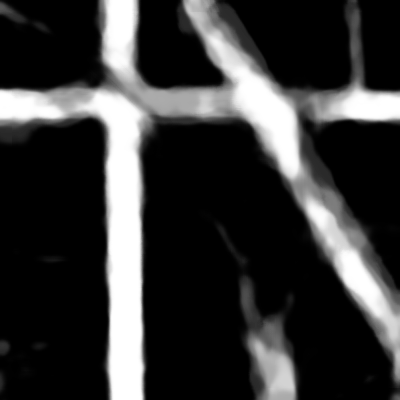
\includegraphics[width=\columnwidth]{figures/training_hard/eval_probability_pred_003.png}
    \end{subfigure}
     \begin{subfigure}[b]{0.3\columnwidth}
      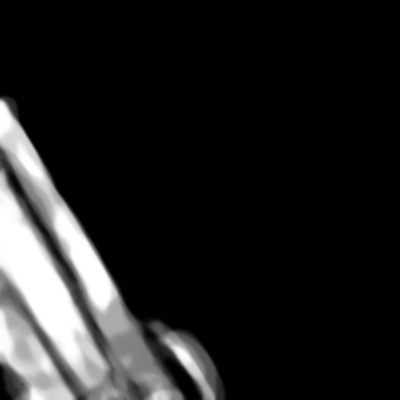
\includegraphics[width=\columnwidth]{figures/training_hard/eval_probability_pred_004.png}
    \end{subfigure}
    \caption{Training evaluation: \textbf{Row 1}: original image with predicted road probability overlay in red. \textbf{Row 2}: ground truth \textbf{Row 3}: classification errors, \textbf{Row 4}: road probability intensity}\label{fig:train_eval}
\end{figure}

\begin{figure}
    \centering
    \begin{subfigure}[b]{0.45\columnwidth}
        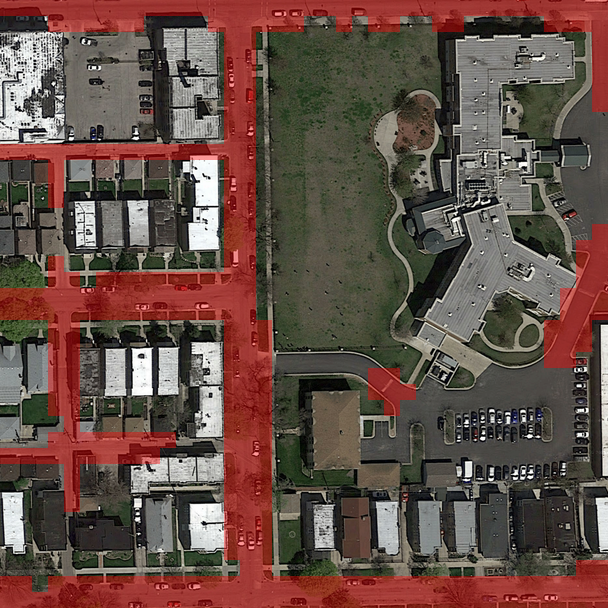
\includegraphics[width=\columnwidth]{figures/submission_selection/images_003.png}
    \caption{Image 3}\label{fig:sub_a}
    \end{subfigure}
    \begin{subfigure}[b]{0.45\columnwidth}
        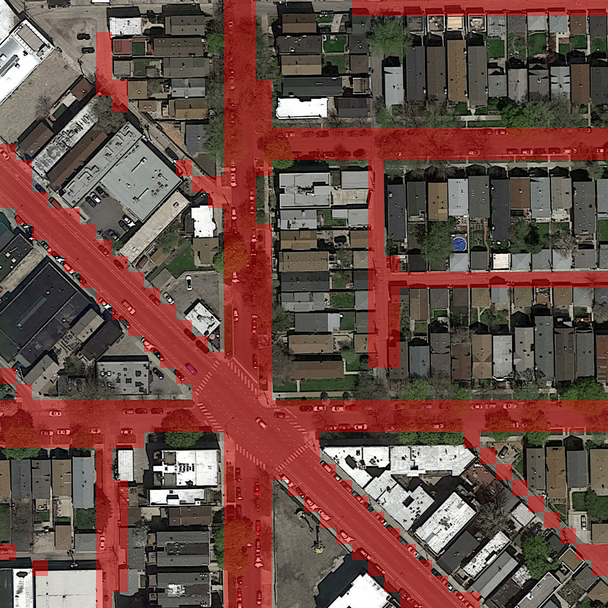
\includegraphics[width=\columnwidth]{figures/submission_selection/images_014.png}
    \caption{Image 14}\label{fig:sub_b}
    \end{subfigure}

    \begin{subfigure}[b]{0.45\columnwidth}
      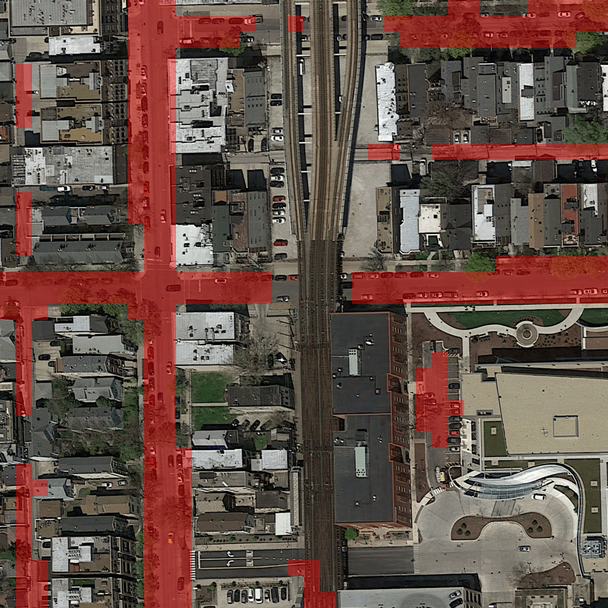
\includegraphics[width=\columnwidth]{figures/submission_selection/images_022.png}
      \caption{Image 22}\label{fig:sub_c}
    \end{subfigure}
    \begin{subfigure}[b]{0.45\columnwidth}
      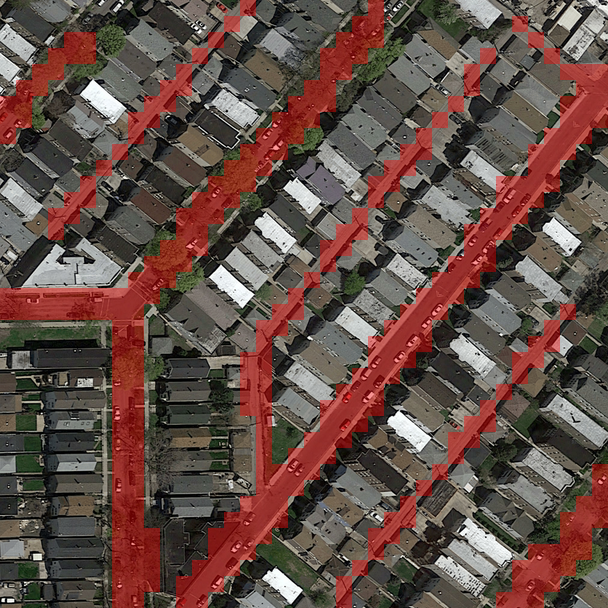
\includegraphics[width=\columnwidth]{figures/submission_selection/images_048.png}
      \caption{Image 48}\label{fig:sub_d}
    \end{subfigure}

\caption{Selection of submitted pictures with road prediction as overlay.}\label{fig:submission}
\end{figure}


\section{Ensemble Prediction}\label{sec:ensemble}
Since our network sees the training images in different perspectives, predictions can be made from different angles. By enabling the ensemble prediction, the system generates $90, 180$ and $270$ degrees rotations, as well as horizontal and vertical flips over the middle axes. This results in 6 predictions for each image. The final prediction is computed by inverting the transformations and averaging the probabilities derived from pixel-wise logits. This is an expensive trick, that multiplies the prediction time by 6 and makes only a marginal improvement in accuracy. We keep it for the sake of the improved result, but taking only one prediction would be enough for a good result and a better fit for production use case.

\section{Software Architecture}\label{sec:implementation}
We used Tensorflow (\citealt{tensorflow2015-whitepaper}) to define our computation graph. Tensorboard was used for metrics visualization and to decide when to stop the training. We trained our model on a single Nvidia GeForce Titan X for about 5 hours. Prediction takes approximately 6 seconds per image of size $608\times608$. We encountered some memory explosion during data augmentation, which prevented us to increase the size of the model. That is the reason why we opted for online stochastic data augmentation when possible in TensorFlow.

\begin{table}[H]
\begin{center}
\begin{tabular}{l|c|c|c|c|c|c|c|c|c}
\textbf{Name} & $p_{drop}$ & 45$^{\circ}$ & m-rot & SA & L & EP & DI & t & $f_1$ \\
\hline
Baseline        & 0   & - & - & - & - & - & - & ? & 0.804\\
U-Net Vanilla   & 0.2 & - & - & - & 5 & - & - & 9 & 0.926\\
U-Net Kiwi      & 0.2 & \checkmark & - & - & 5 & - & - & 6 & 0.932\\
U-Net Apple     & 0.2 & \checkmark & \checkmark & - & 5 & - & - & 9 & 0.935\\
U-Net Guava     & 0.2 & \checkmark & \checkmark & \checkmark & 5 & \checkmark & - & 4 & 0.935\\
U-Net Lime      & 0.2 & \checkmark & \checkmark & \checkmark & 6 & \checkmark & - & 9 & 0.936\\
U-Net Mango   & 0.0 & \checkmark & \checkmark & \checkmark & 6 & \checkmark & \checkmark & 8 & \textbf{0.939}\\
\end{tabular}
\captionof{table}{$\mathbf{p_{drop}}$: dropout probability, $\mathbf{45^{\circ}}$: simple rotation (200 images total), \textbf{m-rot}: rotations~\ref{sec:rotation} $\rightarrow$ implies 45$^{\circ}$, \textbf{SA}: stochastic augmentation~\ref{sec:aug}, \textbf{EP}: Ensemble prediction~\ref{sec:ensemble}, \textbf{DI}: dilated convolutions, \textbf{t}: training time in hours, $\mathbf{f_1}$: test score on Kaggle}\label{tbl:results}
\end{center}
\end{table}

\section{Results}\label{sec:results}

We went through an iterative process of parameter tweaking. The biggest improvements we witnessed were due to data augmentation, particularly the 45 degree rotation augmentation. The impact on evaluation image (\cref{fig:sub_d}) was impressive, around +0.8 F1 point. It is explained by the under representation of diagonal roads in the training dataset, that are easily simulated with rotations.

The effect of dropout remains not completely explained, it helped training but the results on unseen images were better without it (while it is supposed to play the role of a regularizer). We retrained our model without dropout to improve the results.

Early stopping was applied whenever the prediction scores of unseen images were decreasing. The stochastic data augmentation was able to delay this overfit behavior slightly, but it did not prevent it. Table~\ref{tbl:results} shows the evolution of our model and our most important results. UN Guava is our final version with the best obtained Kaggle score.

Figure~\ref{fig:submission} shows four selected submission pictures. Overall, streets are captured very well. Small streets are interrupted sometimes. This is visible on all four sample submission pictures. Additionally, shadows of buildings seem to be a further difficulty. This phenomenon is visible for example on image~\ref{fig:sub_a} on the upper left. The shadow causes a part of the street not to be captured. Trees may cause the same issue. Figure \ref{fig:sub_c} shows the lack of recognition of streets covered by other structures like bridges. Furthermore, on the bottom of the same figure a large piece of road is not recognized at all, most likely because of its darker appearance.

\section{Discussion \& future work}\label{sec:discussion}

We used a powerful model that is well suited for image segmentation. The novelty is very limited, but we gathered and implemented state of the art techniques from different image segmentation papers. It was a bit frustrating to fight for 0.1 percent improvement for the sake of the ranking. Other tasks could have been more meaningful: reducing the size of the model to deploy it on embedded systems, tackle noisy or obstructed images, segmenting different types of roads (e.g.\ mountain roads in Switzerland, paths in Eastern Asia), learning a multi-class model for roads, houses, green spaces, cars\ldots The definition of road can be tricky but it seems that road segmentation is almost a solved problem, the model is sometimes even better than naive humans.

\bibliographystyle{apalike}
\bibliography{literature}

\end{document}
